\documentclass[aspectratio=1610, handout]{beamer}
%\linespread{1.5}\selectfont

\usepackage{booktabs}
\usepackage{dcolumn}
\usepackage{float}
\usepackage{placeins}
\usepackage{lscape} 
\usepackage{tikz}
\usepackage[export]{adjustbox}
\usepackage{ragged2e}
\justifying
\usepackage{outlines}
\usepackage{amsmath}
\usepackage{booktabs}
\usepackage{float}
\usepackage{dcolumn}
\usepackage{longtable}
\usepackage{array}
\usepackage{multirow}
\usepackage{wrapfig}
\usepackage{float}
\usepackage{colortbl}
\usepackage{pdflscape}
\usepackage{tabu}
\usepackage{threeparttable}
\usepackage{caption}
%\captionsetup{font=footnotesize}
\usepackage{subcaption}
\usepackage{threeparttable}
\usepackage[normalem]{ulem}
\usepackage{makecell}
\usepackage{xcolor}
\usepackage{hyperref}
\hypersetup{
    colorlinks = true, 
    linkcolor = red, 
    urlcolor = teal, 
    citecolor = blue}

%\usepackage{caption}
%\captionsetup{labelformat=empty}
\usepackage{appendixnumberbeamer}

\DeclareUnicodeCharacter{0301}{\'{e}}
\DeclareUnicodeCharacter{2212}{-}
\DeclareUnicodeCharacter{0327}{\c}

\usepackage[backend = biber, style=authoryear, sorting = nty, maxcitenames=1]{biblatex}

\addbibresource{citations_sesmarias.bib}

\graphicspath{{~/OneDrive - University of Illinois - Urbana/Research/Projects/Sesmarias Brazil/Figures/Descriptive/}}

%\addbibresource[location = remote]{https://raw.githubusercontent.com/ViniOkadaSilva/Papers/master/Sesmarias/citations_sesmarias.bib}

\DeclareFieldFormat{citehyperref}{%
  \DeclareFieldAlias{bibhyperref}{noformat}% Avoid nested links
  \bibhyperref{#1}}

\DeclareFieldFormat{textcitehyperref}{%
  \DeclareFieldAlias{bibhyperref}{noformat}% Avoid nested links
  \bibhyperref{%
    #1%
    \ifbool{cbx:parens}
      {\bibcloseparen\global\boolfalse{cbx:parens}}
      {}}}

\savebibmacro{cite}
\savebibmacro{textcite}

\renewbibmacro*{cite}{%
  \printtext[citehyperref]{%
    \restorebibmacro{cite}%
    \usebibmacro{cite}}}

\renewbibmacro*{textcite}{%
  \ifboolexpr{
    ( not test {\iffieldundef{prenote}} and
      test {\ifnumequal{\value{citecount}}{1}} )
    or
    ( not test {\iffieldundef{postnote}} and
      test {\ifnumequal{\value{citecount}}{\value{citetotal}}} )
  }
    {\DeclareFieldAlias{textcitehyperref}{noformat}}
    {}%
  \printtext[textcitehyperref]{%
    \restorebibmacro{textcite}%
    \usebibmacro{textcite}}}

\renewcommand*{\nameyeardelim}{\addcomma\space}

\usepackage{setspace}
\usepackage{graphicx}

\newcommand{\tinytable}[1]{\textcolor{black}{\tiny \input{#1}}}

\graphicspath{{~/OneDrive - University of Illinois - Urbana/Research/Writing/git/Sesmarias/Pictures/}}

\beamertemplatenavigationsymbolsempty

%Information to be included in the title page:
\title{Colonial Portuguese Land Grants in Brazil: Long-term Effects on Inequality and Economic Development}
\author{Vinicius Okada da Silva}
\institute{The University of Illinois at Urbana-Champaign}
\date{}

\setbeamertemplate{footline}[frame number]

\begin{document}


\begin{frame}[plain, noframenumbering]
	\titlepage
\end{frame}

\begin{frame}{Motivation}
    \begin{outline}
        \1 Inequality, in both land and income, is high in Brazil.
            \2 ``Brazil has one of the highest levels of inequality of land distribution in the world. Inadequate access to land by the poor and insecure land tenure are factors behind rural poverty violence, human rights abuses, and exploitation of rural workers in conditions of servitude'' \parencite{Usaid2016-xs}
            \2 ``An estimated 1\% of the population owns 45\% of all land in Brazil. Nearly five million families are landless.'' \parencite{Usaid2016-xs}
            % \2 This can be traced even back in history, based on the 1920 census (add quote here about inequality in 1920)
        \pause 
        \1 How much of it can be traced to colonial institutions?
            \2 Goal of this research would analyze the effects of the Portuguese \textit{sesmarias} land grants on long-term inequality in Brazil.
    \end{outline}
\end{frame}

\begin{frame}{History/Background}
    \begin{outline}
        \1 Originally a medieval Portuguese Law used to grant lands to be used and developed \parencite[p.~16]{Diegues_Junior1959-ba}
        \1 First mention of it in Brazil was in 1530, and often favored the Portuguese aristocracy \parencites[p.~16]{Diegues_Junior1959-ba}{Lobb1976-mc}
            \2 Often very large with early ones up to 2,000 $km^2$ \parencite{Nozoe2006-hj}.
            \2 Early studies argued it led to the development of the ``economic aristocracy of the colonial society'' and the ``principal cause of the \textit{latifundio}'' in Brazil \parencites[p.~36]{Lima2002-kd}[p.~48]{Da_Costa_Porto1979-dz}.
            \2 ``Today the system of ownership and use of land is a continuation of the colonial system, with the \textit{sesmaria} becoming \textit{latifundia} property" \parencite[p.~18]{Andrade1980-md}.
    \end{outline}
\end{frame}

\begin{frame}{History/Background}
    \begin{outline}
        \1 Officially stopped being granted in 1822 shortly before Brazil's independence \parencite{Silva2019-vj}. 
        \1 Land reform in Brazil came under a new regime in 1850 with the \textit{Lei das Terras} \parencite[p.~148]{Da_Costa_Porto1979-dz}
            \2 \textit{Sesmeiros} who had owned land and had developed it would be able to retain their lands, however, if not taken care of they would be retaken by the government.
            \2 However, the land reform did not mean the end of the local political power of land owners \parencite{Motta1998-xw}.
    \end{outline}    
\end{frame}

\begin{frame}{Research Question}
    \begin{outline}
        \1 What are the long-term economic effects of the \textit{sesmarias} land grants in Brazil?
            \2 Land inequality $\Rightarrow$ only those with sufficient financial conditions were granted \textit{sesmarias}, and were often granted vast plots of land.
            \2 Income inequality $\Rightarrow$ land was associated with wealth, fewer people with land lead to wealth accumulation by the few.
            \2 Demographic Differences $\Rightarrow$ \textit{Sesmarias} often required African slaves, which could skew the demographics of a location.
            \2 Economic Development $\Rightarrow$ often the lands granted were developed by the owners, leading to the early economic development of an area.
            %\2 Urban development $\Rightarrow$ .
            \2 Political corruption: Dominance by aristocrats often hampered efforts for local reform and investment.\footnote[frame,1]{``If the land was concentrated by a few owners, the \textit{latifundio} is created and it limits the number of settlers and the possibility of them entering the social class of \textit{senhores de engenho} or farmers \parencite[p.~40]{Bandecchi1963-uj}}
    \end{outline}
\end{frame}

\begin{frame}{Literature Review}
    \begin{outline}
        \1 Role of colonization and land tenure in present outcomes:
            \2 Brazil: \cites{Naritomi2012-or}{Musacchio2014-pq}{Wigton-Jones2020-ex}{Laudares2022-vy}
            \2 India: \cites{Banerjee2005-ki}
            \2 Africa: \cites{Lowes2020-pr}
    \end{outline}
\end{frame}

\begin{frame}{Data}
    \begin{outline}
        \1 Brazilian Censuses (1872-2010)
            \2 Possibility of exploring other demographic data from other sources (eg. \href{http://colonialpopulations.fcsh.unl.pt/mainEnglish.php}{Counting Colonial Populations})
        \1 Brazilian Agricultural Censuses (First one in 1920 (?)).
        \1 Location of \textit{sesmarias} from \href{http://plataformasilb.cchla.ufrn.br/}{Sesmarias of the Luso-Brazilian Empire Database}.
    \end{outline}
\end{frame}

\begin{frame}{Example of Document}
    \begin{figure}
        \centering
        \begin{subfigure}[t]{0.35\textwidth}
        \centering
        \vspace{-7.4cm}
        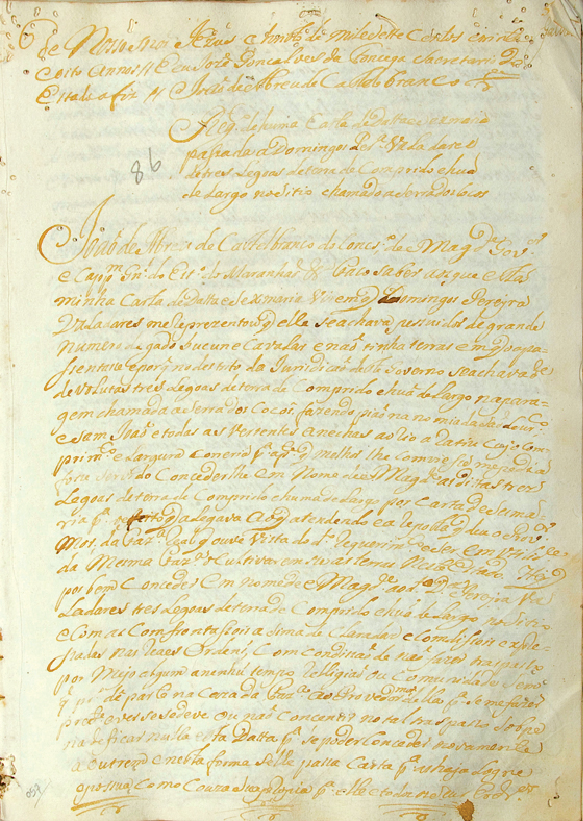
\includegraphics[width = \textwidth]
        {0167f614a7c3b3fd38127f1545dbee7c.pdf}
        \end{subfigure}
        \hspace{0.2cm}
        \qquad\tikz[baseline=-\baselineskip]\draw[ultra thick,->] (0,4) -- ++ (1,0);\qquad
        \hspace{-0.25cm}
        \begin{subfigure}[t]{0.4\textwidth}
        \centering
        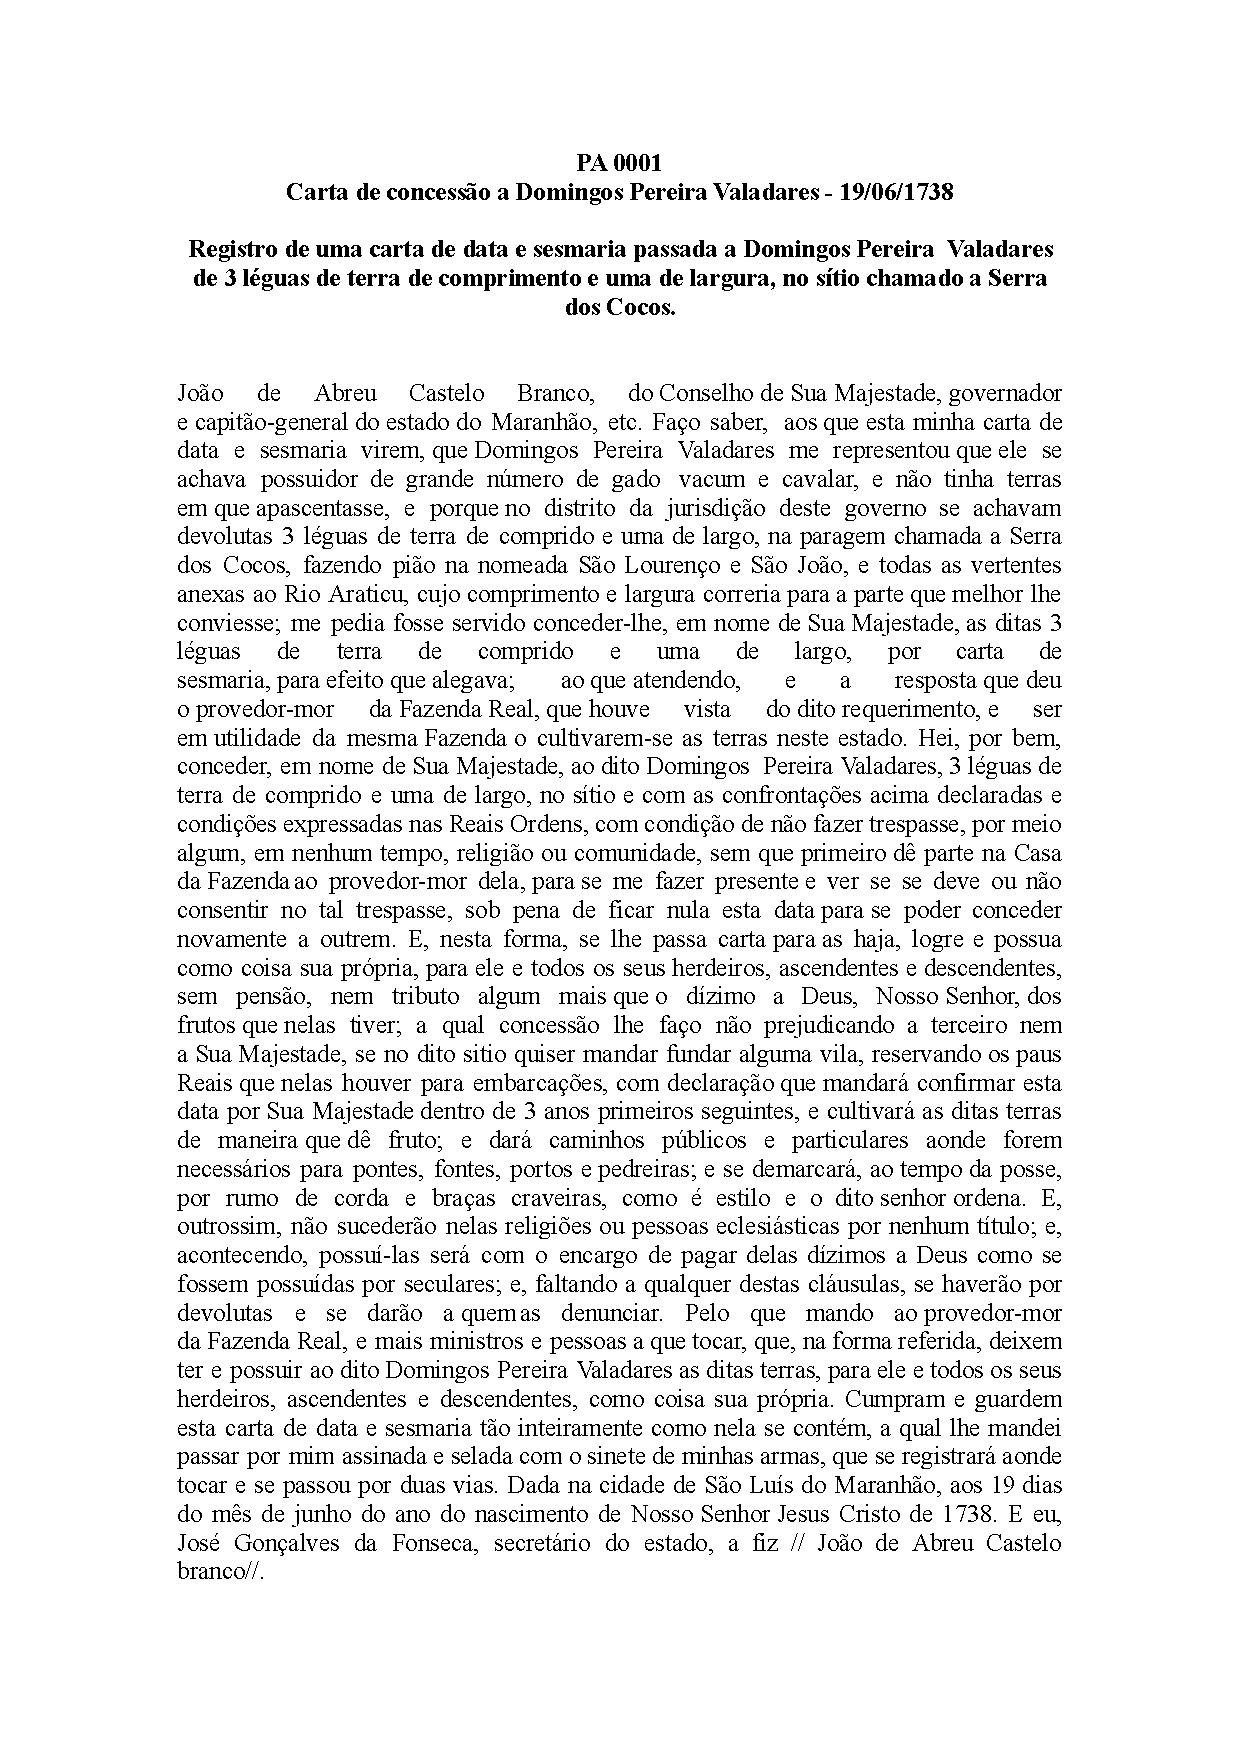
\includegraphics[page = 1, width = \textwidth]
        {ea71ea6ac7c5ec3cefa24ded60ac6438.pdf}
        \end{subfigure}
    \end{figure}
\end{frame}

% Need to create here beamer buttons so people can zoom in if they want.

% \begin{frame}{Information Extraction}
% \end{frame}

\begin{frame}{Identification/Possible Sources of Variation}
    Unsure exactly what's the best way for identification. Below are some of the variation that can be obtained from the data:
    \begin{outline}
        \1 Geographical Variation.
        \1 Time Variation.
        \1 Type of Settler to whom it was granted.
        % \1 Concessions vs. Applications
        \1 What purpose was the land requested (cattle, sugar plantation/factory, etc.).
    \end{outline}
\end{frame}

\begin{frame}{Work to be Done}
    \begin{outline}
        \1 Transcription of Manuscripts and information extraction are being done in Brazil.
            \2 Four states in the Northeast will be finished by March.
            \2 My state of \href{https://www.rosepepe.com.br/hotsite_acervo/sesmarias/}{Para} (\href{http://www.siaapm.cultura.mg.gov.br/modules/brtbusca/index.php?action=results&query=sesmarias&x=-722&y=-59}{and Minas Gerais}) has all the transcriptions $\Rightarrow$ only needed to extract the information.
                \3 Machine Learning techniques to extract the information (?)
        \1 Georeferencing would be most of the work required.
            \2 By myself, try creating a group, or looking for professional help?
    \end{outline}
\end{frame}

\begin{frame}{Basic Descriptive Statistics}{Land History}
    \centering
    \includegraphics[width=0.85\textwidth,height=0.85\textheight,keepaspectratio]
    {~/OneDrive - University of Illinois - Urbana/Research/Projects/Sesmarias Brazil/Figures/Descriptive/land_type.png}
\end{frame}

\begin{frame}{Basic Descriptive Statistics}{Year Dist.}
    \centering
    \includegraphics[width=0.85\textwidth,height=0.85\textheight,keepaspectratio]
    {~/OneDrive - University of Illinois - Urbana/Research/Projects/Sesmarias Brazil/Figures/Descriptive/year_dist.png}
\end{frame}

\begin{frame}{Basic Descriptive Statistics}{Size Dist.}
    \centering
    \includegraphics[width=0.85\textwidth,height=0.85\textheight,keepaspectratio]
    {~/OneDrive - University of Illinois - Urbana/Research/Projects/Sesmarias Brazil/Figures/Descriptive/size_dist.png}
\end{frame}

\begin{frame}{Other Angles}
    \begin{outline}
        \1 Possible to focus only where we would expect them to have an effect and spend time transcribing/focusing on them (eg. Northeast).
            \2 ``Under the auspices of King Philip I (1581-1598), the \textit{sesmaria} was widely applied in the northeast and central coast regions of Brazil where a system involving large properties and slave labor was considered the only way to make a profit in the new land, whether by means of cultivation or cattle ranching.''\parencite{Lobb1976-mc}
            \2 Sugarcane plantations required extensive amounts of slave labor \parencites{Silva2019-vj}[p.~16]{Baer2014-gh}.
            \2 ``Much of the windfall profits of the sugar cycle had been appropriated by Portuguese and foreign intermediaries, whereas a large part of the profits accruing to the \textit{fazenda} and \textit{engenho} owners were spent on imported consumer goods rather than technical and infrastructural improvements'' \parencite[p.~16]{Baer2014-gh}
    \end{outline}
\end{frame}

\begin{frame}{Other Relevant (?) Information to Add}
    \begin{outline}
        \1 Sesmarias caused economic uncertainty in colonial times as often poor people would settle, develop land, and then lose the right of the land because a richer person would claim it \parencite[p.~142]{Da_Costa_Porto1979-dz}.
    \end{outline}
\end{frame}

\begin{frame}[allowframebreaks, t, noframenumbering, plain]{References}
    \printbibliography
\end{frame}

\appendix


\end{document}